
\subsection{1.33 Соединения со связью металл-металл, кластеры. Природа связи, геометрия молекул. Способы получения, химическое поведение.}
Определение по Коттону: \noindent \\
Кластеры — это соединения, которые содержат ограниченное число атомов металлов, которые связаны ковалентными связями друг с другом полностью или в значительной степени, даже если имеются дополнительно атомы неметаллов (лиганды), связанные с кластером. \\ \\
Для того, чтобы была связь $M_M$ необходимы:
\begin{itemize}
	\item Низкая степень окисления
	\item Большой атомный номер
\end{itemize}
Большие выступающие орбитали металла будут хорошо перекрываться. \\
Связи $M-M$ слабые по энергии, бывают одинарные и кратные\\
\begin{figure} [H]
	\centering {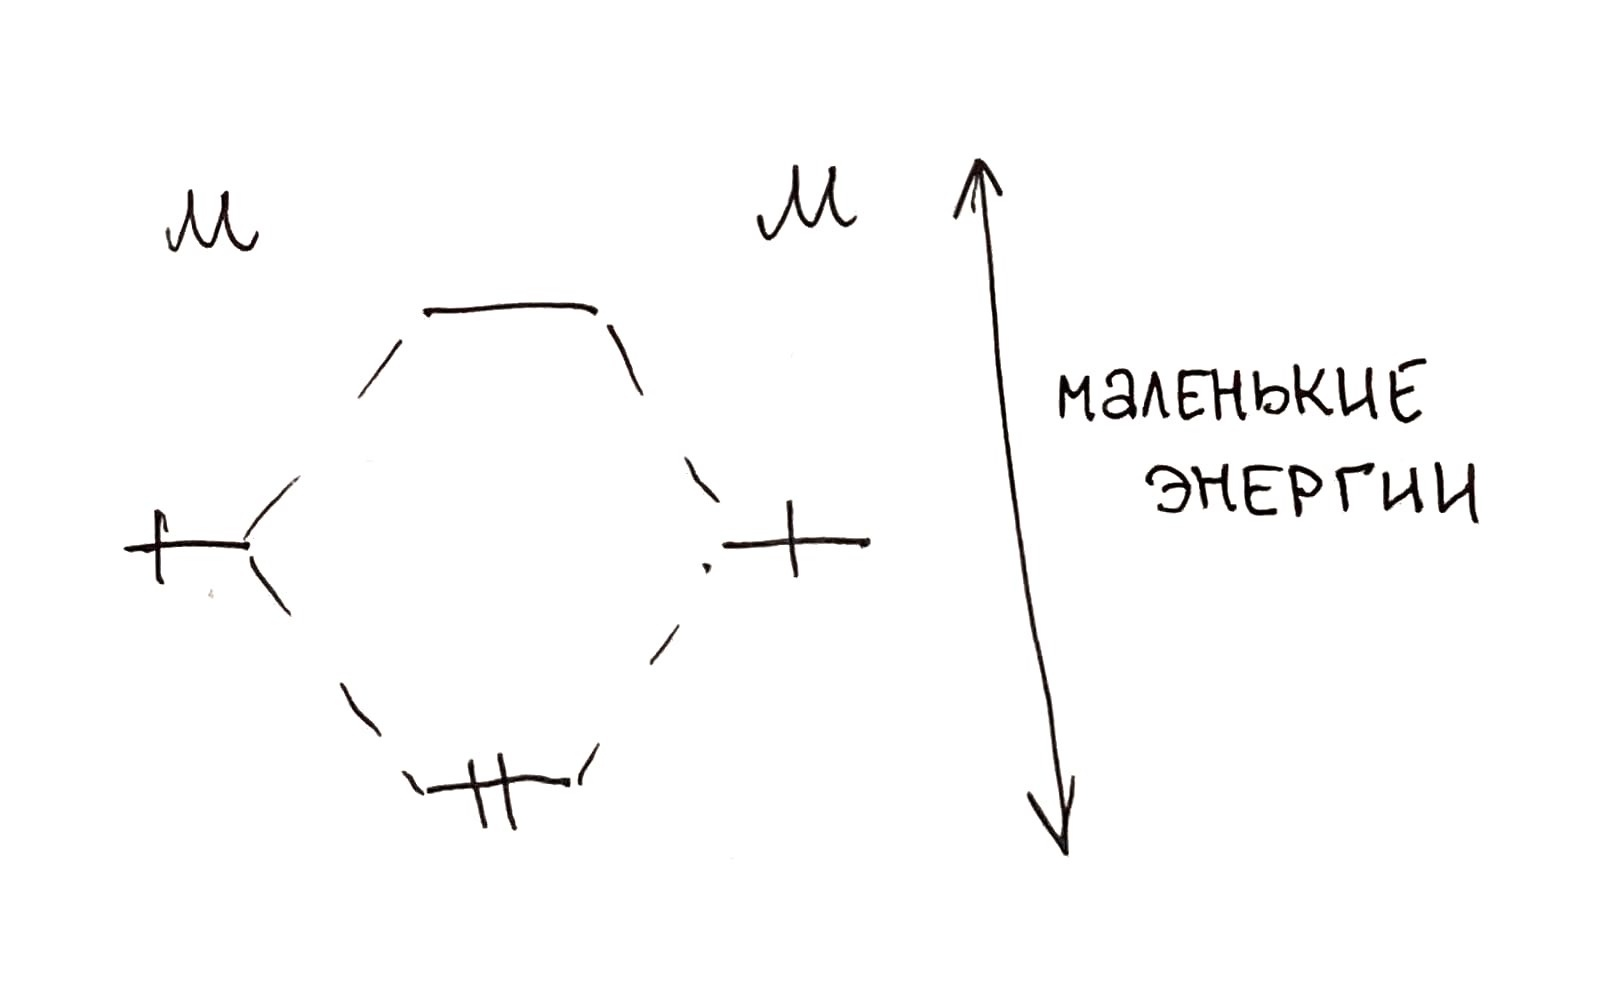
\includegraphics[scale=0.15]{ff2}}
\end{figure}
\textbf{Геометрия молекул}\\
Различные полиэдры, основные типы:
\begin{figure} [H]
	\centering {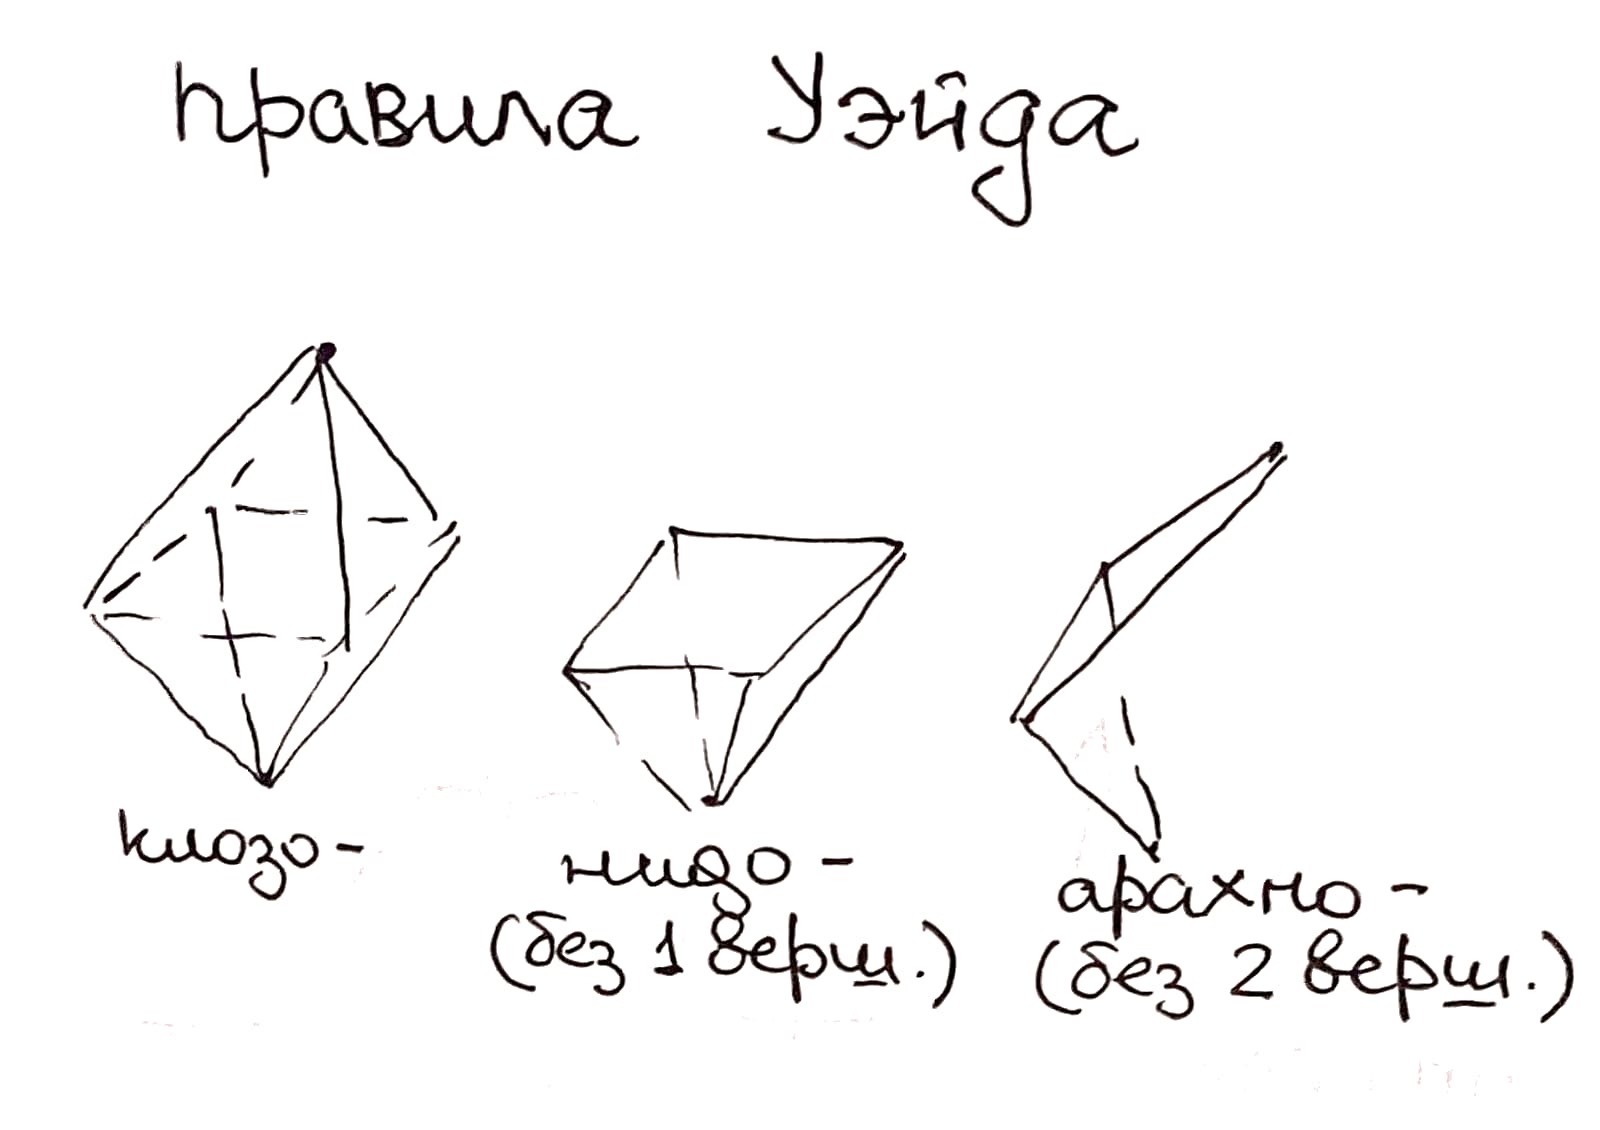
\includegraphics[scale=0.15]{ff1}}
\end{figure}
Правила Уэйда позволяют связать геометрию кластера с его электронным строением. \\
Принцип изолобальности: одинаковые характеристики граничных орбиталей, симметрия, число электронов, энергия \\
\begin{figure} [H]
	\centering {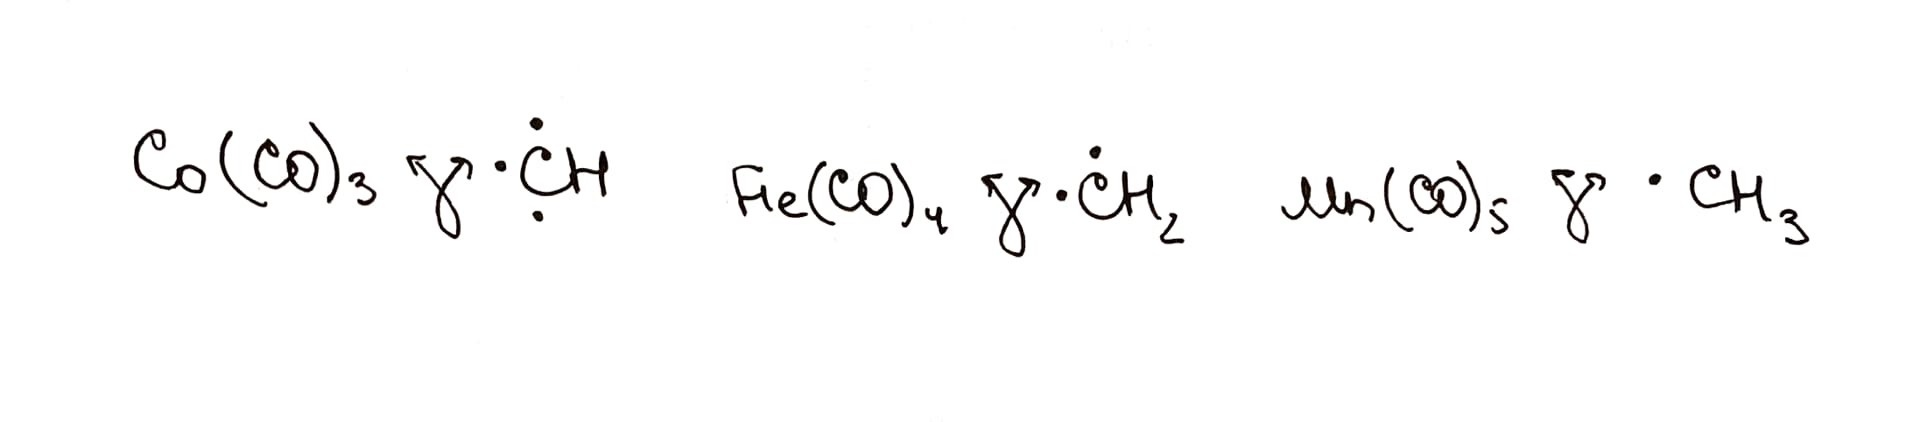
\includegraphics[scale=0.15]{ff3}}
\end{figure}
Определенное число электронов $\Rightarrow$ определенная геометрия \\
\textbf{Получение и свойства}
\begin{itemize}
	\item $Co(CO)_4 + AgNO_3 = (AgCo(CO)_4)_4 $
	\item $ Ru_3(CO)_{12} + \left[ Fe(CO)_4 \right]^{2-} = H^+ = H_2FeRu_3(CO)_{13} $
	\item $Os_3(CO)_{12} = t = Os_5(CO)_{16} + Os_6(CO)_{18} + Os_7(CO)_{21} ... $
	\item $ Fe(CO)_5 \rightarrow Fe_2(CO)_9 = t, HC\equiv CH = Fe_2(CO)_{15}C $ \\ имеет форму квадратной пирамиды, где в вершинах пирамиды $Fe$, а в центре основания - $C$
	\item $ Na_2Fe(CO)_4 + Fe(CO)_5 + NO^+BF_4^- = H^+ = HFe_5(CO)_{14}N $
	\begin{figure} [H]
		\centering {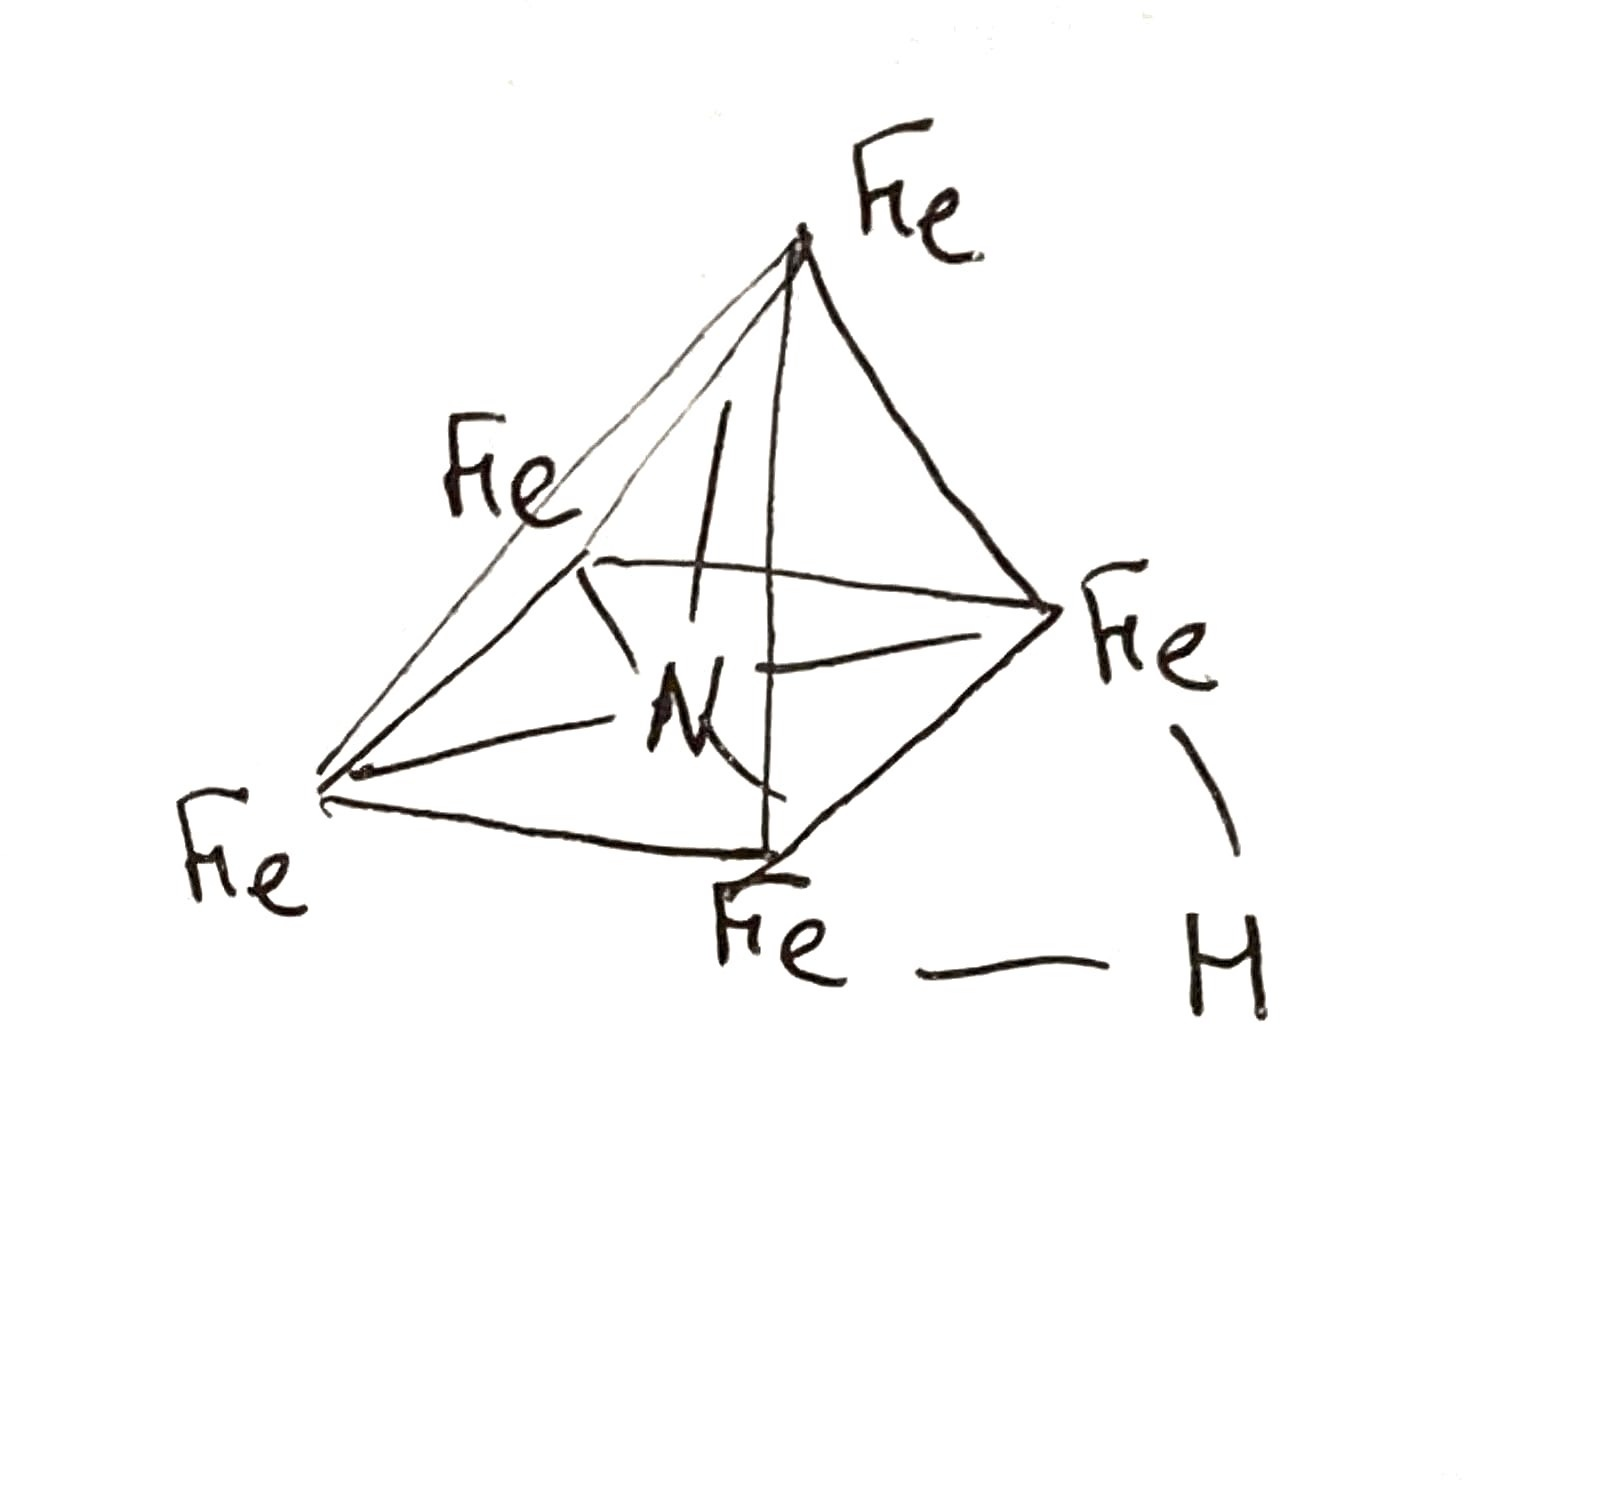
\includegraphics[scale=0.15]{ff4}}
	\end{figure}
\end{itemize}
